
\paragraph{Control system selection}
Based on the arguments for and against certain control system concepts given in Chapter \ref{subsec:controltool} a selection of suitable control system solutions was made. Figure \ref{fig:cgoffset} shows the \gls{cg} offset required along the Z-axis to trim the spacecraft at certain angles of attack for various \gls{cg} locations on the X-axis. 
\begin{figure}[ht]
	\centering
	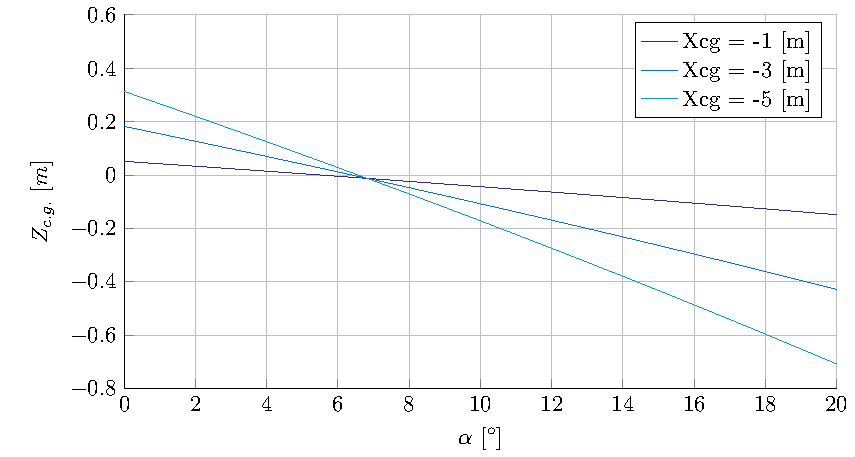
\includegraphics[width=0.95\textwidth]{./Figure/control/moment}
	\caption{\acrlong{cg} offset along Z-axis required for a trimmed condition at various angles of attack}
	\label{fig:cgoffset}
\end{figure}
From Figure \ref{fig:cgoffset} it can be seen that the required \gls{cg} Z-offset grows as the X-offset grows. For an angle of attack change of $2$ degrees corresponding to an X-\gls{cg} located at $-5$ meters a \gls{cg} shift of $0.2$ meters is required. Angle of attack-based trajectory control was found to require trimmed \gls{sym:alpha}-shifts of $5$ degrees that have to be adjusted with a rate of $1$ $[deg \cdot s^{-1}]$. To pull this off would require the actuation system to produce a \gls{cg} displacement of $0.5$ meters with a required rate of $0.1$ $[m \cdot s^{-1}]$. This would require excessively heavy actuators that would also have to be able to operate under 3-g loads. Not only has this never been done before in space at such scale, the reliability of such a system would be questionable as a \gls{spf} would be introduced. Based on these arguments a decision was made against active \gls{cg} control.\\
Following the decision to discontinue the consideration of active \gls{cg} control a selection had to be made between the other two control system design options: Body flaps and thrusters. Regarding body flaps some of the same arguments can be made as were used against active \gls{cg} control. Body flaps can require excessively large actuators that are very heavy. In addition to this the dynamic behaviour of the inflatable structure is difficult to compute and can be very unpredictable. Furthermore the use of body flaps on inflatable structures has a very low \acrlong{trl}, which poses an additional development risk. Based on these and other downsides pertaining to aerodynamic control surfaces mentioned in Chapter \ref{subsec:controltool} it was decided to employ thrusters as control system.

\paragraph{Control system actuation}

The components of the control system providing the actuation can globally be subdivided into two components. The control system mass and its corresponding accuracy.

Mass estimates are based on the required propellant mass, thruster mass and fuel tank mass. The propellant mass can be subdivided into a further two categories: the control within the atmosphere and the control outside of the atmosphere. General equation were previously discussed within Chapter \ref{subsec:controltool}. An overview of the mass components and their respective masses is provided in Table \ref{tab:controlmassbreakdown}.

\subparagraph{Control within the atmosphere} 

Within the Martian atmosphere control is performed on the basis of banking. A control system featuring a single bank control reversal manoeuvre is always able to derive at the destination with a average accuracy of $1.009$ $[km]$ at Mars\cite{Lu2007}. The control system accuracy can further be significantly reduced by using multiple bank reversals. Reductions are primarily found in the observed dispersions.

Accuracies using bank control where obtained using dispersions of $\pm 0.03 $ \gls{sym:CL}, $\pm 0.06 $ \gls{sym:CD} and mass and atmospheric dispersion of $5\%$ and $30\%$ respectively \cite{Lu2007}. Accuracies of up to $10$ $[m]$ can be achieved if the staging and final descent are included \cite{Davis2010}. These control accuracies were obtained on the basis of sensed accelerations.

It is argued that with an increasing amount of bank reversals, complemented with additional control measures such as extra sensors, higher accuracies can be obtained. The trajectories are budgeted for a total of six bank reversals, three for both the initial aero-capture and the final \gls{edl}. Three bank reversals are typical values for single orbit \cite{Lu2007, Cianciolo2010}. A very qualitative definition of three bank reversals as defined within the control system analysis is displayed in Figure \ref{fig:bankdef}.

\begin{figure}[h]
	\centering
	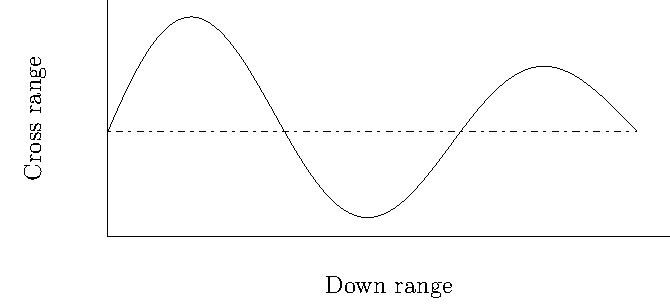
\includegraphics[width=0.6\textwidth]{./Figure/control/Cont.pdf}
	\caption{Qualitative figure displaying three bank reversals}
	\label{fig:bankdef}
\end{figure}s

The mass estimates of the propellant required within the Martian atmosphere are based on peak rotational rates of $20$ $[deg\cdot s^{-1}]$ and $5$ $[deg \cdot s^{-2}]$ as used by Davis et al. \cite{Davis2010}.

The inertial moments are based on a homogeneous mass distribution and a simplified geometric shape. The crew module is assumed to be a hollow cylinder with the structural components attached to the in and outside of this cylinder. The inflatable structure is assumed to be of a circular disk shape, again with a homogeneous mass distribution. Within this shape the mass is assumed to be primarily situated on the outside of the spacecraft such that a conservative mass estimates will be achieved.

\subparagraph{Control outside the atmosphere}
Control outside the Martian atmosphere is required for two purposes. Clean-up corrections and orbit (de)-raising. The latter allows for a controlled entry time into the Martian atmosphere for the final \gls{edl} operations. The former makes sure that the desired orbit can be reached after the aerobraking.

For the purpose of orbit raising it is desired that the consequential orbit no longer covers the Martian atmosphere and that the orbital period fits within a Martian day. For practical purposes and considering the relatively short period in space (i.e. days) after the initial aerocapture the pericenter limit is set at 200 $[km]$. 

Clean-up corrections are estimated based on results presented by Cianciolo et al. \cite{Cianciolo2010}. The most representative shapes are the $23$ meter diameter \gls{hiad} and in lesser extend the rigid aeroshell. On the basis of the former the clean-up velocity are estimated to be $10.47$ $[m\cdot s^{-1}]$ ($3\sigma$) \cite[p.37]{Cianciolo2010}. Note that Cianciolo et al. include the orbit raising within the clean-up estimates whereas this report considers them as two separate entities.


\subparagraph{Thrusters}
Inertial moments combined with rotational rates deliver the required control moments via Equation \ref{eq:mcontrol}. For the most efficient performance the thruster are placed on the outside of the crew module. Although thrusters placed on the outside of the inflatable are able to generate higher torques, multiple disadvantages hinder this placement:
\begin{itemize}
\item Thruster placed on the inflatable will difficult the deployment
\item Deformation of the inflatable, and thus thruster performance, is difficult to predict.
\item Placement of thrusters on the inflatable may induce disadvantageous vibrations or aero-elastic effects.  
\end{itemize} 

Further details on the placement are also discussed in Chapter \ref{sec:crewpackaging} discussing the packaging of the re-entry vehicle.

Thruster performance requirements are primarily based on the bank control speed. Apocenter velocity increments may take longer but are however also greater in magnitude. The thrusters used for creating the bank control moments require a peak thrust of around $900$ $[N]$. Torque is provided by multiple thrusters such that partial operations may continue if a thruster fails.
Indicative values for a capable thruster are for example given by the  MONARC-445 hydrazine mono-propellant thruster\footnote{URL: \url{http://www.moog.com/literature/Space\_Defense/Spacecraft/Propulsion/Monopropellant\_Thrusters\_Rev\_0613.pdf} Accessed 15 June 2015}. The MONARC-445 thruster delivers a nominal thrust of $445$ $[N]$ at a mass of 1.6 $[kg]$.  A configuration with eight of these thrusters allows for control around the roll axis and moreover provides partial control in the case of failure of one such thruster.
 
Specific preference lies in the use of hydrazine as propellant such that it is interchangeable with the remaining propellent requiring systems. The use of a single propellant allows for lower fuel fractions as propellants margins required for the different mission phases can be combined.

Additionally thrusters for the velocity increments in the apocenter are required. Again hydrazine thrusters are considered for interchangeability throughout the various mission stages. This is however combined with a second propellent as bi-propellant thrusters yield significant performance increases (in terms of \gls{sym:Isp}) \cite{Wertz2011}. 

A thruster suitable for such a purpose is the Apogee kick engine by IHI Japan at a mass of $15.7$ $[kg]$ and a specific impulse of $321.4$ $[s]$. As secondary propellant \gls{nto} is required \cite[p.538]{Wertz2011}. This thruster can only be used if placed aft of the re-entry vehicle, since the front is covered by the \gls{hiad} additional pointing by the crew module \gls{adcs} system may be required. To ensure sufficient control system reliability two of these thrusters will be employed so that no \acrfull{spf} can occur. 

\begin{table}[h]
	\centering
\caption{Overview of thruster properties}
\label{tab:thrusters}
\hspace{-5mm}
\begin{tabular}{|p{0.12\textwidth}|p{0.16\textwidth}|p{0.04\textwidth}|p{0.06\textwidth}|p{0.08\textwidth}|p{0.14\textwidth}|p{0.13\textwidth}|l|} \hline 
\textbf{Engine    }          &\textbf{ Manufacturer }         & \textbf{Qt.} &\textbf{Mass $\mathbf{[kg]}$}      & \textbf{Length $\mathbf{[m]}$} & \textbf{Propellants}  & \textbf{Nominal Thrust $\mathbf{[N]}$} & \textbf{\gls{sym:Isp} $\mathbf{[s]}$} \\ \hline \hline
MONARC 445          & MOOG                  & 8        & 1.6  & 0.41 & Hydrazine     & 445         & 321.4   \\ \hline
Apogee kick engine & IHI Japan Company Ltd. & 2        & 15.7 & 1.03 & \gls{nto}/ ~~~~~ Hydrazine & 1700        & 235.0     \\ \hline
\end{tabular}
\end{table}


\subparagraph{Propellant tanks}
One of the main arguments for the use of hydrazine as the primary propellant is the ability to combine the propellent budgets for multiple mission phases as previously mentioned. This allows for a lower control system mass fractions as for an equal control system reliability. Nevertheless a mass estimate for the propellent tank is provided to yield a fair mass estimate for the \gls{hiad} design. 

The tank mass is estimated via the empirical Equation \ref{eq:tankmass} \cite[p. 543]{Wertz2011}.

\begin{equation}
\label{eq:tankmass} 
\gls{sym:m}_{tank}=2.7086 \cdot 10^{-8} \cdot \gls{sym:vol}^3 -6.1703 \cdot 10^{-5} \cdot \gls{sym:vol}^2 +6.66290 \cdot 10^{-2}  \cdot \gls{sym:vol} +1.3192;
\end{equation}

\subparagraph{Component mass overview}

Table \ref{tab:controlmassbreakdown} provides an overview of the individual mass components discussed above. Mass estimates exclude the final contingency factor of $20\%$ applicable for all the \gls{hiad} components.

\begin{table}[h]
\centering
\caption{Control system mass components}
\label{tab:controlmassbreakdown}
\begin{tabular}{|l|l|c|} \hline
\textbf{Component}           &\textbf{$\Delta V$}  & \textbf{Mass $\mathbf{[kg]}$} \\ \hline \hline
Bank Control    &  - &			 66       \\ \hline
Clean-up         & 10.47  &		  33       \\ \hline
Orbit (de)raising& 18.12  &		  54       \\ \hline
Fuel tank              		 & -  &  12      \\ \hline
Thrusters                	 & -  &  44     \\ \hline \hline
\textbf{Total}               & -  &  212      \\ \hline
\end{tabular}
\end{table}

\paragraph{Control system method}

For achieving mission success it is essential that required accuracy can be obtained even under non nominal conditions. For this purpose a control system is required such that the bank reversal angles and timing can be properly chosen such that a reference trajectory can be followed and the mission succeeds.

Similar to the mass estimates the control system can  also be subdivided into part within and a part outside of the Martian atmosphere.

\subparagraph{Control within the atmosphere}

Control within the atmosphere is required in two phases of the mission. The initial aero capture phase and the final \gls{edl}. Due to small uncertainties in the \glspl{hiad} performance, but more importantly atmospheric disturbances, deviations from the nominal trajectory can be observed. These deviations are accounted for in the trajectory discussed in Section \ref{sec:trajectorydesign} but also need to be recognised during mission operations such that they can be acted upon. 

Typical implementations for a control system involve a \gls{npc} or \gls{apc} method and use sensed accelerations to determine the atmospheric properties \cite{Davis2010}. These values are used to update the control models such that the same terminal point is reached each time. For this purpose a set of three gyroscopes and three accelerators as \gls{imu} is required \cite{Dutta2013}. The former is already included in the \gls{adcs} as discussed in Chapter \ref{subsec:adcs}. Recent advances in accelerometers make even the high accuracy sensors a low mass component. The accelerometers are included in the \gls{adcs} mass budget as they are also required for the terminal descent phase. 

For achieving the high required landing accuracy it is advised that next to sensed accelerations to determine the control model parameters pressure sensors are included as well.  \gls{npc} and \gls{apc} methods for bank control on Mars do normally not include these sensors and merely rely on sensed acceleration data \cite{Lu2007, Davis2010}. Since pressure can not be measured directly during the hypersonic flight use is made of flush atmospheric data \cite{Dutta2013}. 
 
Such sensors are demonstrated in hypersonic flight in the \gls{msl} in 2012 \cite{Dutta2013}. The use of separate sensors for determining the atmospheric properties will allow for easier determination of the atmospheric properties and allow for a higher landing accuracy on order to meet the set requirements. A very schematic overview of the functioning of the control system within the atmosphere is given in Figure \ref{fig:Contsys}.

Normal model update frequencies, using only sensed accelerations, are in the order of 10 seconds \cite{Davis2010}. The usage of the additional pressure sensors allow for more frequent model updates as changes are more easily observed again benefiting the accuracy of the control system.

\begin{figure}[h]
	\centering
	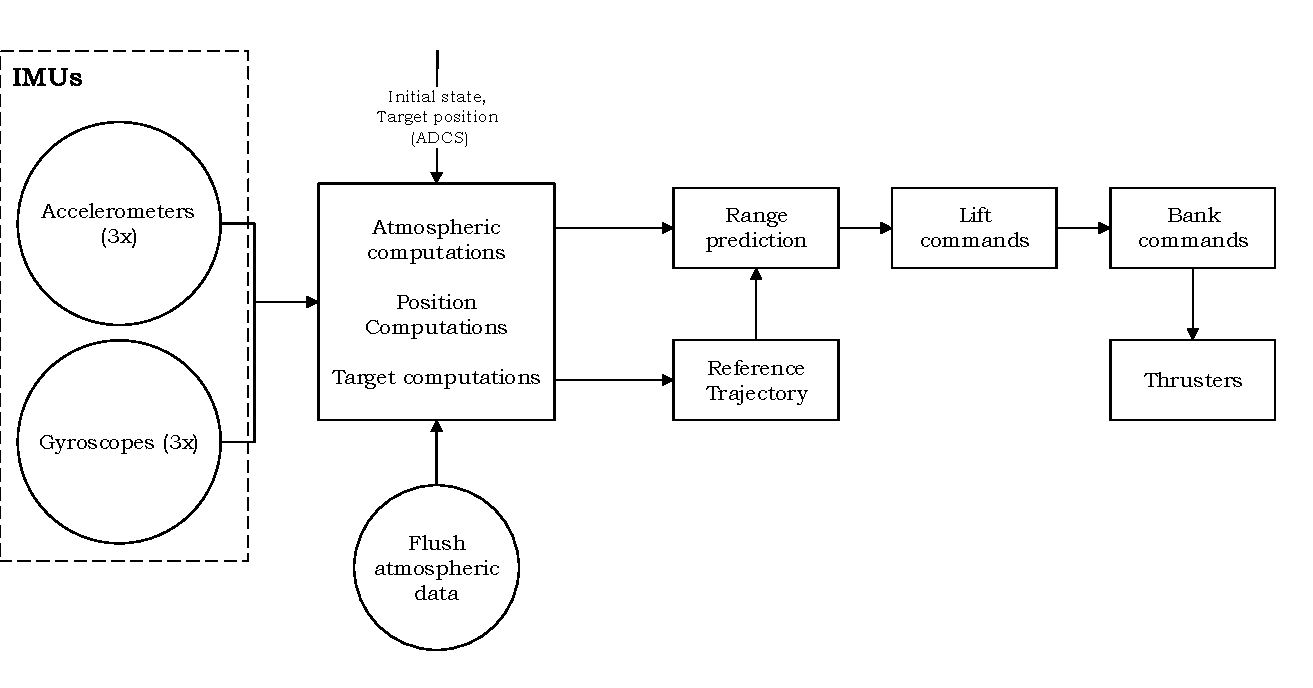
\includegraphics[width=0.95\textwidth]{./Figure/control/Contsys.pdf}
	\caption{A schematic overview of the control system functioning}
	\label{fig:Contsys}
\end{figure}

\subparagraph{Control outside the atmosphere}

Outside the Martian atmosphere no additional sensors are required apart form those provided by the \gls{adcs}. The period outside the Martian atmosphere however serves as an aid for the final \gls{edl}. Unlike the initial aero capture phase, for which no timing is possible, the period outside the Martian atmosphere in between the two entries allows for additional measurements and control model updates. Moreover the timing of the second re-entry in the Martian atmosphere can be controlled in intervals of single Martian days.

Controlling this entry allows for entries at favourable atmospheric conditions and reduces the risk of the mission. Atmospheric conditions can for example be transmitted via pre-existing base stations. Controlling the timing of the mission allows for much more certainty on the atmospheric conditions which is crucial for the precision of the re-entry. High variations in the atmospheric properties, such as may be the case due to for example dust storms me be prevented \cite{Justh2012}.


